\section{Desarrollo de la propuesta}

Como ya se ha mencionado vamos a diseñar un circuito basado en multiplicadores 
de tensión o duplicadores de Greinacher para conseguir a la salida los $3kV$ 
especificados. 

En primer lugar, vamos a calcular cuántas celdas duplicadoras son necesarias 
en el diseño para obtener los $3kV$ a la salida. Para ello hay que tener en cuenta que el condensador 
de salida de
cada celda duplicadora se carga a una tensión igual al doble de la tensión de pico de la fuente, por lo que 
al poner varias celdas en serie, la tensión entre el terminal positivo del último condensador 
y la referencia (terminal negativo de la fuente) se irá duplicando. Por tanto, el cálculo 
queda de la siguiente manera:
\begin{equation}
    \text{nº duplicadores} = \frac{3000\,V}{220\cdot\sqrt{2}\cdot2} = 4.821 \approx 5
\end{equation}

Por tanto, con cinco duplicadores de tensión podemos obtener los $3kV$ de continua a partir 
de la fuente de $220 V_{rms}$. 
\begin{figure}[H]
    \centering
    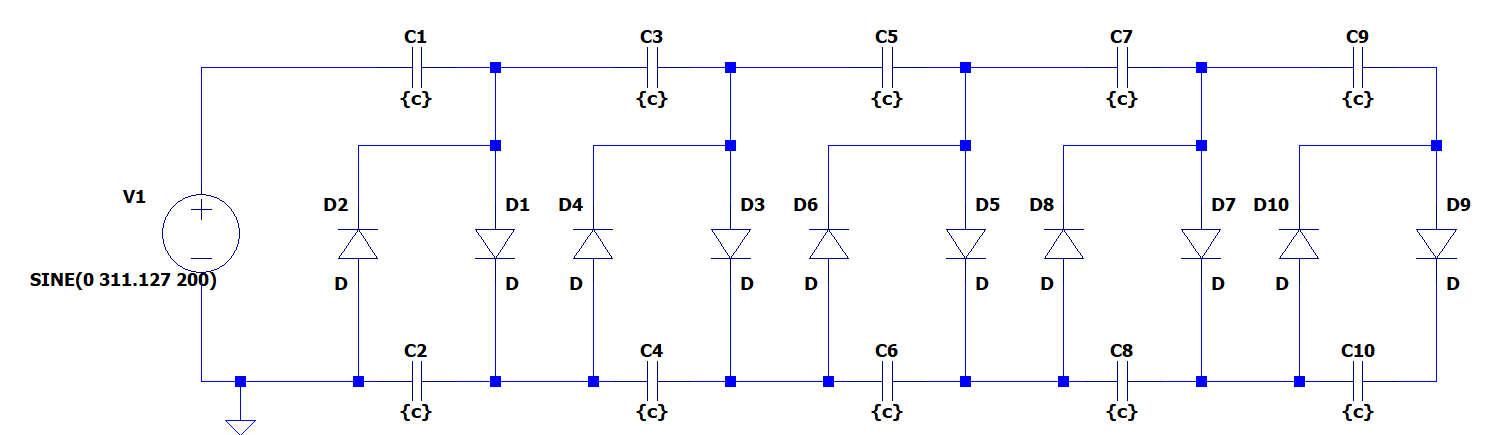
\includegraphics[width=0.9\textwidth]{img/mult_final.png}
    \caption{Esquema con los multiplicadores necesarios}
    \label{fig:esquema_mult}
\end{figure}

Con este esquema, idealmente y sin carga tendremos a la salida la siguiente tensión:
\begin{equation}
    V = 5\cdot2\cdot220\cdot\sqrt{2} = 3111.27\,V
\end{equation}

Por otro lado, la corriente de salida del circuito multiplicador tiene que se 
aproximadamente de $5 mA$. Para conseguir esta corriente de salida tenemos que calcular 
una carga que se conecte a la salida del multiplicador y que consuma esa corriente, ya que el multiplicador 
aislado, una vez se han cargado todos los condensadores, no consume ninguna corriente. La carga 
se puede calcular fácilmente mediante la Ley de Ohm:
\begin{equation}
    V = R\cdot I \rightarrow R = \frac{V}{I} = \frac{5\cdot2\cdot220\cdot\sqrt{2}}{0.005} = 622254\,\Omega
\end{equation}

Este consumo de corriente provoca que los condensadores se descarguen más rápidamente, aumentando 
el rizado y provocando una caída de tensión final, por lo que hay que emplear unos condensadores con 
una capacidad lo suficientemente elevada para minimizar el rizado y la caída de tensión. Además, esto producirá que el consumo de corriente
de la carga no sea exactamente igual al calculado, pero se asumirá este error puesto que el rizado y la caída de tensión son dependientes de la frecuencia
y el circuito debe ser capaz de funcionar en un rango de $50Hz$ a $200Hz$.

Como se ha mencionado en las especificaciones, el rizado máximo debe ser de un $\pm20\%$. En este caso 
realizaremos el diseño para tener un rizado de pico a pico de aproximadamente $10V$, que sería un 
rizado de aproximadamente $\pm8\%$. Para la obtención del rizado vamos a comenzar calculándolo 
en el supuesto de que solo tuviésemos una celda duplicadora. Si llamamos $t_1$ al tiempo en el que conduce el diodo que carga 
el condensador en cada ciclo y $t_2$ al tiempo en el que no conduce el diodo, es decir, el tiempo de descarga 
del condensador en cada ciclo, podemos expresar la corriente que el condensador aporta a la carga $R$ de la siguiente forma (llamamos 
q a la carga transferida en cada ciclo):
\begin{equation}
    I = \frac{dq}{dt} \approx \frac{q}{t_2}
\end{equation}

Como pasado el transitorio el tiempo $t_1$ es mucho menor que $t_2$ podemos aproximar 
$t_2$ de la siguiente forma:
\begin{equation}
    t_2 \approx \frac{1}{f}
\end{equation}

Por otro lado, sabemos que el rizado de tensión en un condensador en función de la carga transferida 
en un ciclo es el siguiente:
\begin{equation}
    \delta V = \frac{q}{C_2}
\end{equation}

Por tanto, combinando las tres ecuaciones anteriores obtenemos la siguiente ecuación:
\begin{equation}
    \delta V = \frac{I}{f\cdot C_2}
\end{equation}

No obstante, en una celda duplicadora, la carga primero se transfiere del condensador $C_1$ al condensador 
$C_2$, por lo que el rizado de pico a pico total a la salida de una sola celda duplicadora será el siguiente:
\begin{equation}
    \delta V = \frac{I}{fC_1}+\frac{2I}{fC_2} = \frac{I}{f}\left[\frac{1}{C_1}+\frac{1}{C_2}\right]
\end{equation}

Extrapolando este resultado a nuestro ejercicio y considerando todos los condensadores iguales con 
una capacidad $C$, el rizado de pico a pico queda de la siguiente forma:
\begin{equation}
    \delta V = \frac{I}{fC}[1+2+3+4+5]=\frac{I}{fC}\cdot15
\end{equation}

Por tanto, para obtener un rizado pico a pico de $10V$, la capacidad de los condensadores debe 
ser la siguiente:
\begin{equation}
    C = \frac{I}{\delta V\cdot f}\cdot15 = \frac{0.005}{10\cdot 50}\cdot 15 = 150\,\mu F
\end{equation}

El cálculo anterior se ha realizado para una frecuencia de $50Hz$ porque es más restrictivo, 
ya que a menor frecuencia mayor rizado. Podemos comprobar el rizado de pico a pico que se obtendrá con ese condensador 
a $200Hz$:
\begin{equation}
    \delta V = \frac{I}{fC}\cdot15 = \frac{0.005}{200\cdot 150\,\mu F}\cdot15 = 2.5\,V
\end{equation}

Por otro lado, podemos calcular la caída de tensión que va a provocar una carga con ese 
consumo de corriente. A partir de la expresión obtenida en la referencia \cite{park2015reduction}:
\begin{equation}
    V_{\text{drop}} = \frac{I}{fC}\left(\frac{2n^3}{3}+\frac{n^2}{2}-\frac{n}{6}\right)
\end{equation}

En la ecuación anterior, $n$ es el número de celdas duplicadoras, por lo que sustituyendo los datos a $50Hz$
la caída del voltaje final es la siguiente:
\begin{equation}
    V_{\text{drop}} = \frac{0.005}{50\cdot 150\,\mu F}\left(\frac{2\cdot5^3}{3}+\frac{5^2}{2}-\frac{5}{6}\right) = 63.33\,V
\end{equation}

Por tanto, el voltaje medio de salida que obtendremos con esa carga a $50Hz$ será el siguiente:
\begin{equation}
    V = 5\cdot2\cdot220\cdot\sqrt{2}-V_{\text{drop}} = 3047.93\,V
\end{equation}

Por otro lado, a $200Hz$ la tensión final será la siguiente:
\begin{equation}
    V_{\text{drop}} = \frac{0.005}{200\cdot 150\,\mu F}\left(\frac{2\cdot5^3}{3}+\frac{5^2}{2}-\frac{5}{6}\right) = 15.83\,V
\end{equation}
\begin{equation}
    V = 5\cdot2\cdot220\cdot\sqrt{2}-15.83= 3095.44\,V
\end{equation}

Por último, nos faltaría el diseño del circuito de medida. Este circuito de medida estará basado en 
un divisor de tensión para poder medir con un fondo de escala de $200V$. Además, la resistencia 
del multímetro es de $10M\Omega$. 

El circuito de medida para el que se van a realizar los cálculos es, por tanto, el siguiente:
\begin{figure}[H]
    \centering
    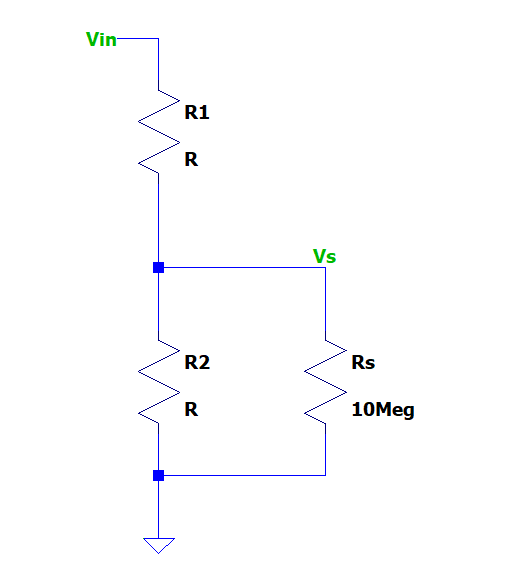
\includegraphics[width=0.4\textwidth]{img/circ_medida.png}
    \caption{Esquema para los cálculos del circuito de medida}
    \label{fig:esquema_med}
\end{figure}

Como valor de $V_{in}$ se selecciona la máxima tensión de salida que el circuito será capaz de proveer y 
dicha tensión se asociará con una caída en $R_2$ y $R_s$ de $200V$. De esta manera, nunca será posible sobrepasar
el fondo de escala. Dicho valor de $V_{in}$ es el siguiente:
\begin{equation}
    V_{in} = 5\cdot2\cdot\sqrt{2}\cdot220 = 3111.27\,V
\end{equation}

Por otro lado, queremos que $V_s$ sea igual a $200V$. Además, $R_2$ en paralelo con $R_s$ debe 
ser menor a 10 $M\Omega$. Si fijamos el valor del paralelo en 9 $\,M\Omega$ (valor elevado para minimizar el consumo del circuito) podemos calcular 
el valor de $R_2$:
\begin{equation}
    \frac{1}{9\,M\Omega} = \frac{1}{10\,M\Omega} +\frac{1}{R_2\,M\Omega} \rightarrow R_2 = 90\,M\Omega
\end{equation}

Por último, obtenemos el valor de $R_1$ a partir del divisor de tensión:
\begin{equation}
    V_s = Vin\cdot\frac{R_2//R_s}{R_1+R_2//R_s} \rightarrow R_1 = \frac{(R_2//R_s)\cdot(V_{in}-V_s)}{V_s}
\end{equation}

Sustituyendo valores, el valor de la resistencia $R_1$ queda:
\begin{equation}
    R_1 = \frac{9\,M\Omega\cdot(3111.27\,V-200\,V)}{200\,V} = 131.007\,M\Omega
\end{equation}

No obstante, uno de los requerimientos de diseño es que los componentes tuviesen una tensión de trabajo 
inferior a $1000V$. En la resistencia $R_1$ en las condiciones de diseño va a caer aproximadamente la siguiente tensión:
\begin{equation}
    V_{R1} = 3111.27\,V-200\,V = 2911.27\,V > 1000\,V
\end{equation}

Por tanto, si dividimos la resistencia $R_1$ en tres resistencias iguales, cada una tendrá una 
tensión de trabajo igual a un tercio de la tensión de trabajo de $R_1$, es decir:
\begin{equation}
    V_{R'} = \frac{V_{R1}}{3} = \frac{2911.27}{3} = 970.42\,V < 1000\,V
\end{equation}

Por tanto, el circuito final del multiplicador de tensión con la carga y el circuito de medida 
de tensión queda de la siguiente manera:
\begin{figure}[H]
    \centering
    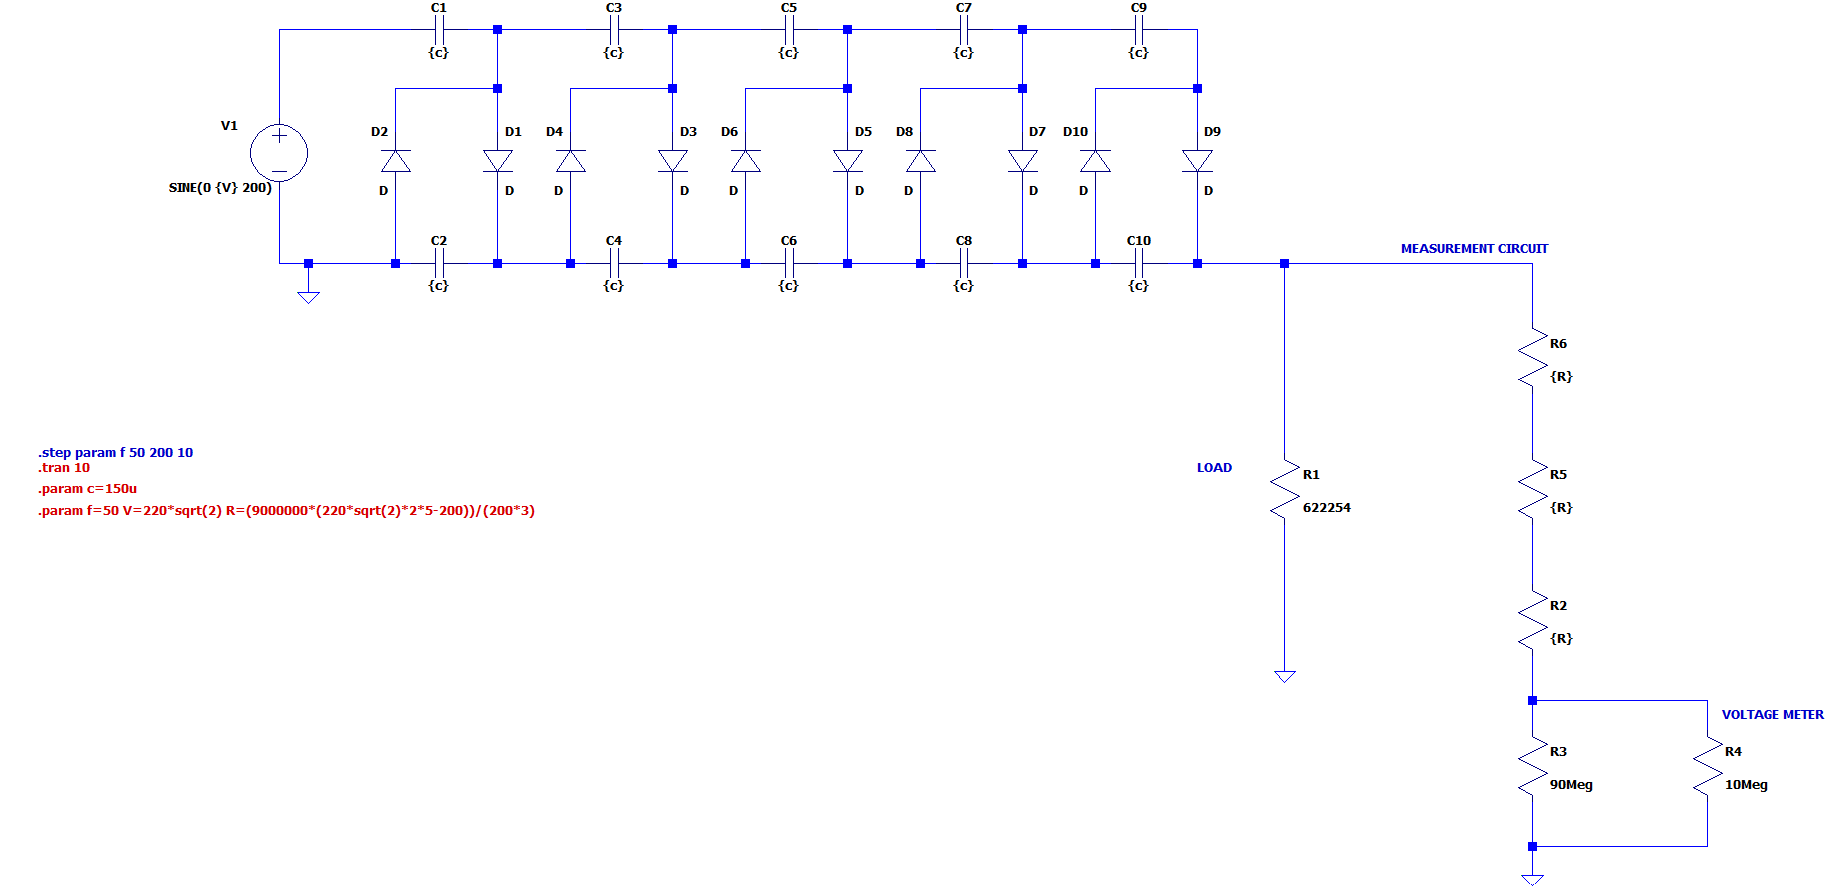
\includegraphics[width=1\textwidth]{img/circ_final.png}
    \caption{Circuito multiplicador de tensión diseñado}
    \label{fig:esquema_final}
\end{figure}

Por último, podemos calcular el consumo de corriente máxima aproximado del circuito de medida\footnote{Nos referimos 
a la corriente máxima que consume el circuito de medida, porque estamos considerando la tensión 
de salida teórica sin caída debido a la carga.}:
\begin{equation}
    I_{meas} = \frac{V_{in}}{R_{total}} = \frac{3111.27}{9\,M\Omega+131.007\,M\Omega} = 22.22\,\mu A
\end{equation}